\chapter{算法设计}
\label{chap3}

\section{算法描述}

\subsection{设计思路}

前面提到现有的算法如果跨路口的两段路出现一段堵车而另一段通行良好的情况,时间会平摊到两段,不够准确。由于算法要求在线,但历史数据可以从服务器端取得,考虑5分钟内路况通常不会出现大的变化,当新的轨迹数据进入系统后,我们可以利用过去五分钟内的历史数据来计算出该轨迹经过路段的准确路况,也保证了算法的在线性。

\subsection{算法优势}

相对于平滑算法,我们对于轨迹数据的利用率更高,能够在相邻道路间速度差异较大时得到比较理想的结果,实现起来也较为简单,算法的复杂度不高,可能很快地计算出结果,能够适应在线系统的要求。模型同样具有可扩展性,只需要简单修改就可以应对多叉路口或者立交桥等复杂路口的情况,也可能扩展到跨越多个路口的情况。

\section{具体实现}

\subsection{模型建立}

\begin{figure}[H] 
  \centering
  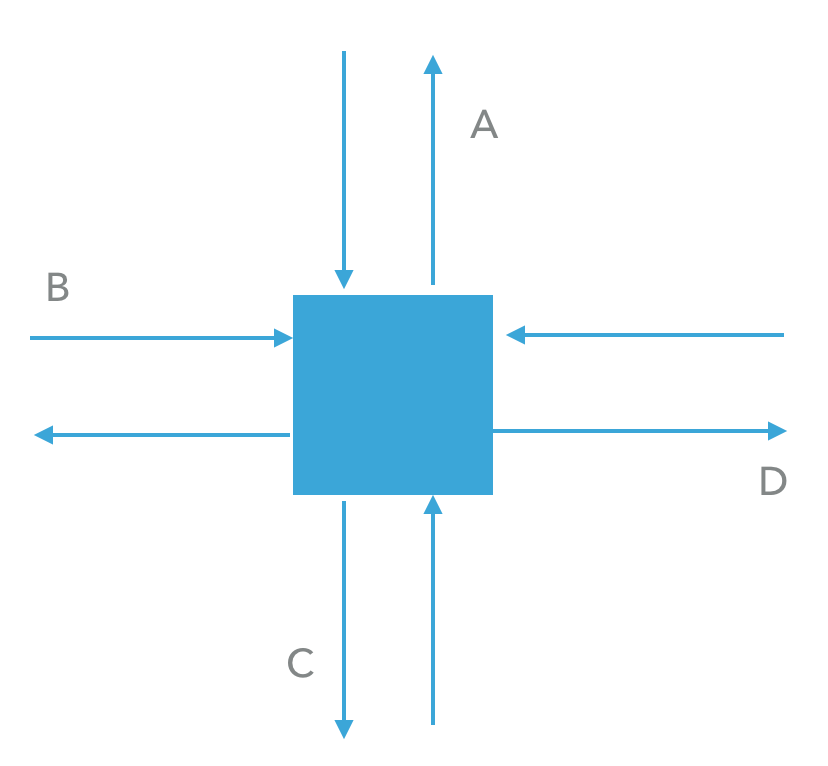
\includegraphics[width=3in]{model_bulid}
  \caption{模型示意图}
  \label{fig:3.1}
\end{figure}

如图\ref{fig:3.1}所示,我们将路口部分抽象成一个黑盒,一个十字路口就被抽象成A,B,C,D4段路径正反8个方向和黑盒中连接这8个方向的12组转向延迟。假设进入十字路口的路段为A1,B1,C1,D1,离开十字路口的则为A2,B2,C2,D2。路口的轨迹数据信息就被抽象成了12组方程。

\begin{equation}
k1_{A1,B2} \times T_{A1} + k2_{A1,B2} \times T_{B2} + turn_{A1,B2} = t_{1}
\end{equation}

\begin{equation*}
k1_{A1,C2} \times T_{A1} + k2_{A1,C2} \times T_{C2} + turn_{A1,C2} = t_{2}
\end{equation*}

......

\begin{equation*}
k1_{D1,C2} \times T_{D1} + k2_{D1,C2} \times T_{C2} + turn_{D1,C2} = t_{12}
\end{equation*}

其中k1与k2是指轨迹覆盖到当前路段的百分比,turn是指该方向的转向延迟,包含花费在交通信号灯或者路口切换装置上的时间,把这些时间加在一起抽象成一个转向延迟的概念。

\subsection{单方向算法}

得到5分钟内的轨迹数据后按照12个方向进行划分,选取出轨迹数量最多的方向先入手。假设该方向5分钟内有n条轨迹,则我们可以得到n组方程,如下所示。再对方程组做线性回归求出拟合直线,之后利用直线的斜率和截距信息计算出花费在第一条路的时间$T_{1}$,花费在第二条路的时间$T_{2}$以及转向延迟turn。

\begin{equation}
\begin{bmatrix}
k_{11}  &  k_{21}   &1\\
k_{12}  &  k_{22}   &1\\
 \vdots   & \vdots   & \vdots  \\
k_{1n}  & k_{2n}    &1\\
\end{bmatrix} \times 
\begin{bmatrix}
T_{1}  \\
T_{2}  \\
turn \\
\end{bmatrix} = 
\begin{bmatrix}
t_{1}  \\
t_{2}  \\
\vdots \\ 
t_{n} \\
\end{bmatrix}
\end{equation}

\subsection{线性回归}
如果数据量多于3条,那么方程是无解的,所以我们需要引入线性回归的算法来近似地得出每段路的路况结果。把总时间$t_{i}$看成随机变量y,把每条道路的通行时间看成自变量$x_{i}$,就有(\ref{f3.1})。

\begin{equation}
y_{i} = \theta^{T}x_{i}+ \epsilon_{i}
\label{f3.1}
\end{equation}

这时使用最小二乘法求出一条使得所有点到拟合直线垂直距离平方之和(\ref{f3.2})最小的拟合直线。

\begin{equation}
\frac{1}{2} \sum_{i=1}^{n} (h_{\theta} (y_{i}-x_{i}))^{2}
\label{f3.2}
\end{equation}

使用最小二乘法对轨迹数据做线性回归也就相当于做了一个最大似然估计,而类似的还有一种方法是使用贝叶斯方法来对轨迹数据做线性回归。Bayes方法的关键是计算后验概率,已知先验分布$p(\theta )= N(0,\tau^{2}I)$之后,我们使用bayes公式得到(\ref{f3.3})

\begin{equation}
p(\theta |S) = \frac{p(S|\theta )p(\theta )}{p(S)} 
\label{f3.3}
\end{equation}

之后以$\theta$为底做积分可以得到y在当前的数据样本空间下的分布(\ref{f3.4}),再对y积分得到线性回归的预测期望值(\ref{f3.5})

\begin{equation}
p(y|x,S)=\int_{\theta}p(y|x,\theta )p(\theta |S)d\theta
\label{f3.4}
\end{equation}

\begin{equation}
E[y|x,S]=\int_{y}p(y|x,S)ydy
\label{f3.5}
\end{equation}

Bayes方法和前面普通的最小二乘法做线性回归最大的区别就是加入了$\theta$的先验概率,也就是要找到使得(\ref{f3.6})最小的拟合直线作为结果。

\begin{equation}
\frac{1}{2} \sum_{i=1}^{n} (h_{\theta} (y_{i}-x_{i}))^{2} + \frac{\theta ^{2}}{2\tau ^{2}}
\label{f3.6}
\end{equation}

bayes方法对比最小二乘法最大的优势就是加入一个先验概率来在一定程度上规避掉过拟合的情况,在图\ref{fig:3.2}中我们选取了一些模拟数据加入了随机的噪声,对比最小二乘法和Bayes方法的效果。

\begin{figure}[H] 
  \centering
  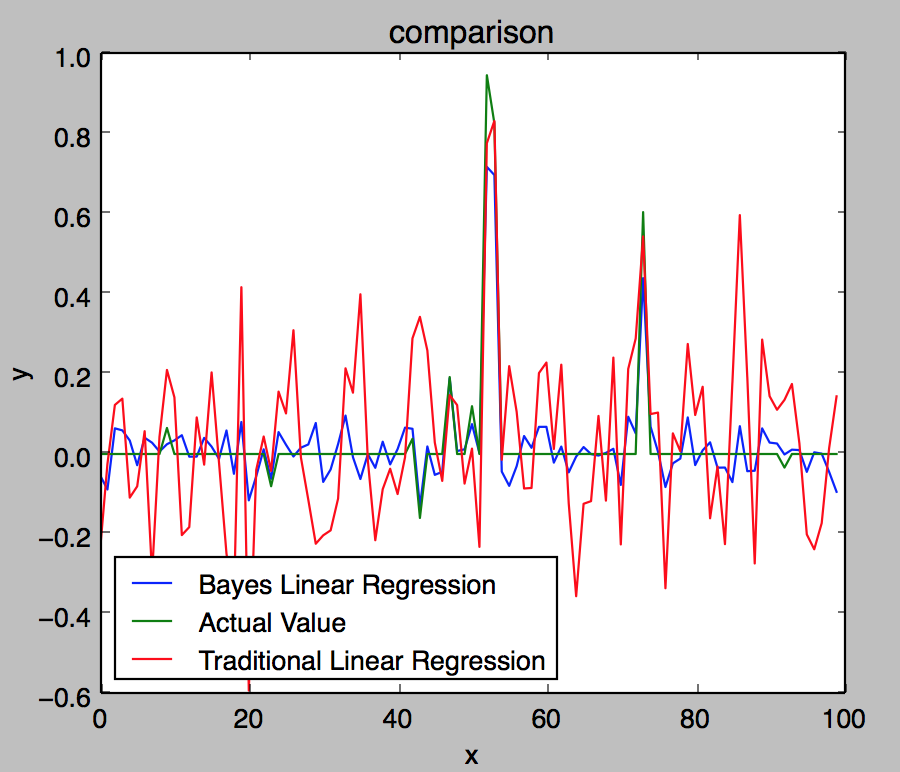
\includegraphics[width=3in]{comparison}
  \caption{Bayes对比最小二乘法}
  \label{fig:3.2}
\end{figure}

图\ref{fig:3.2}中绿色为原始数据,蓝色为Bayes方法回归结果,红色为最小二乘法的回归结果。我们可以看出总体上相比于最小二乘法,Bayes方法回归出的结果更接近于实际值,但是在实际数据中随着数据量的增加,最小二乘法的精确度会比Bayes方法更高,所以我们决定视数据量多少混合使用这两种算法进行计算,具体的结果会在第4章实验部分展示。

\subsection{多方向混合的算法}

考虑通过同一路段的三个方向的轨迹,其中有一条为右转的轨迹,而右转方向通常不需要等待信号灯,结果较为准确,需要的轨迹数量更少,如果可以找到右转的轨迹则先使用右转的轨迹计算得出该路段的路况,之后再结合另外两个方向的轨迹信息求解另外两个方向的路况信息。

对于路口整体的轨迹数据,我们使用相对方向直行和左转一般同时放行,得出相对方向直行和左转的红绿灯周期相同,所以转向延迟相近,计算出到一个方向的路况信息之后可以将转向延迟应用于其对应方向的路况计算,减少数据的需求量,综合这些信息我们设计了一个系统来对路口整体路况做计算,流程图如图\ref{fig:3.3}。

\begin{figure}[H] 
  \centering
  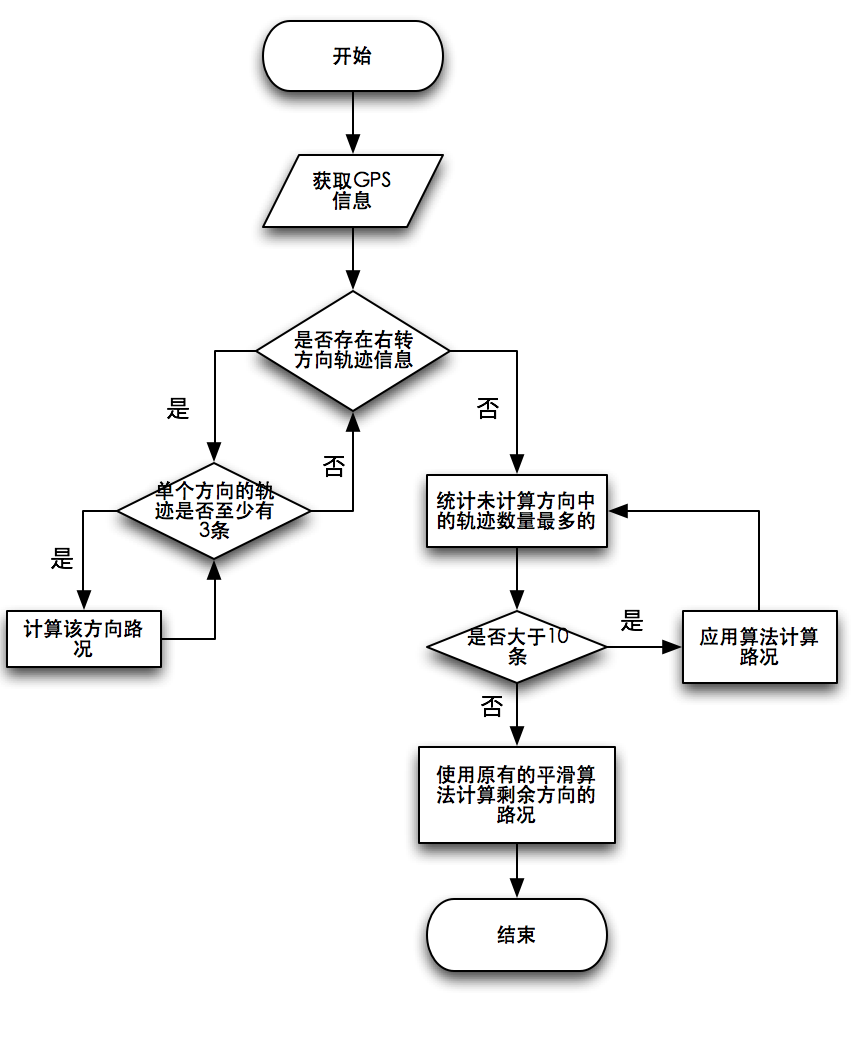
\includegraphics[width=3in]{flowchart}
  \caption{流程图}
  \label{fig:3.3}
\end{figure}

\section{细节改进}

\subsection{细化路口延迟}
为了细化车辆在路口的转向延迟,我们设计了一个方法来计算车辆在路口的等待队列长度,使用静止点序列$A_{n}$的平均值的2倍和和该序列的最大值来估计等待队列长度。
\begin{equation}
waiting\_queue = \max (A_{i}|i=1,2...n,2\times average(A_{n}))
\label{f3.7}
\end{equation}

之后我们细化了路口的转向延迟T(\ref{f3.8})
\begin{equation}
T = t_{2}-t_{1}-|p_{1}-j_{1}|/v_{1}
\label{f3.8}
\end{equation}
其中T为路口延迟,$t_{2}$和$t_{1}$分别是转弯过程中起始和终止点的时间戳,而$|p_{1}-j_{1}|$表示路口等待队列的长度,$v_{1}$是前一段路平滑路段的平均速度。

\subsection{排除异常点}

由于行驶轨迹数据带有一定的随机性,可能出现驾驶员异常操作或道路匹配错误等原因产生的异常数据,所以我们需要将数据中的异常点排除。对于自变量y和拟合向量$\hat{y} = Py$,我们可以得到残差向量$e = y - \hat{y} = (1-P)y$,计算残差平方和$RSS=e^{T}e$进而我们将残差标准化(\ref{f3.12})其中$\hat{\sigma} $为残差的参照值(\ref{f3.11}),假设数据满足正态分布为$N(0,1)$的随机样本,那么$r_{i}$落在$[-2,2]$的概率$P(\mu - 2\sigma < U < (\mu + 2\sigma ) = 95\%$,所以如果$|r_{i}|>2$那么这个点就被视为异常点,将其删除。如图\ref{fig:3.4},该图为一组左转数据的残差图,对于红色的两个点,我们在计算时将其删除,避免对整体结果产生偏差。

\begin{equation}
\hat{\sigma}=\sqrt{RSS/(n-k-1)}
\label{f3.11}
\end{equation}

\begin{equation}
r_{i} = \frac{e_{i}}{\hat{\sigma}\sqrt{1-p_{ii}}}, i = 1,2,...,n
\label{f3.12}
\end{equation}

\begin{figure}[H] 
  \centering
  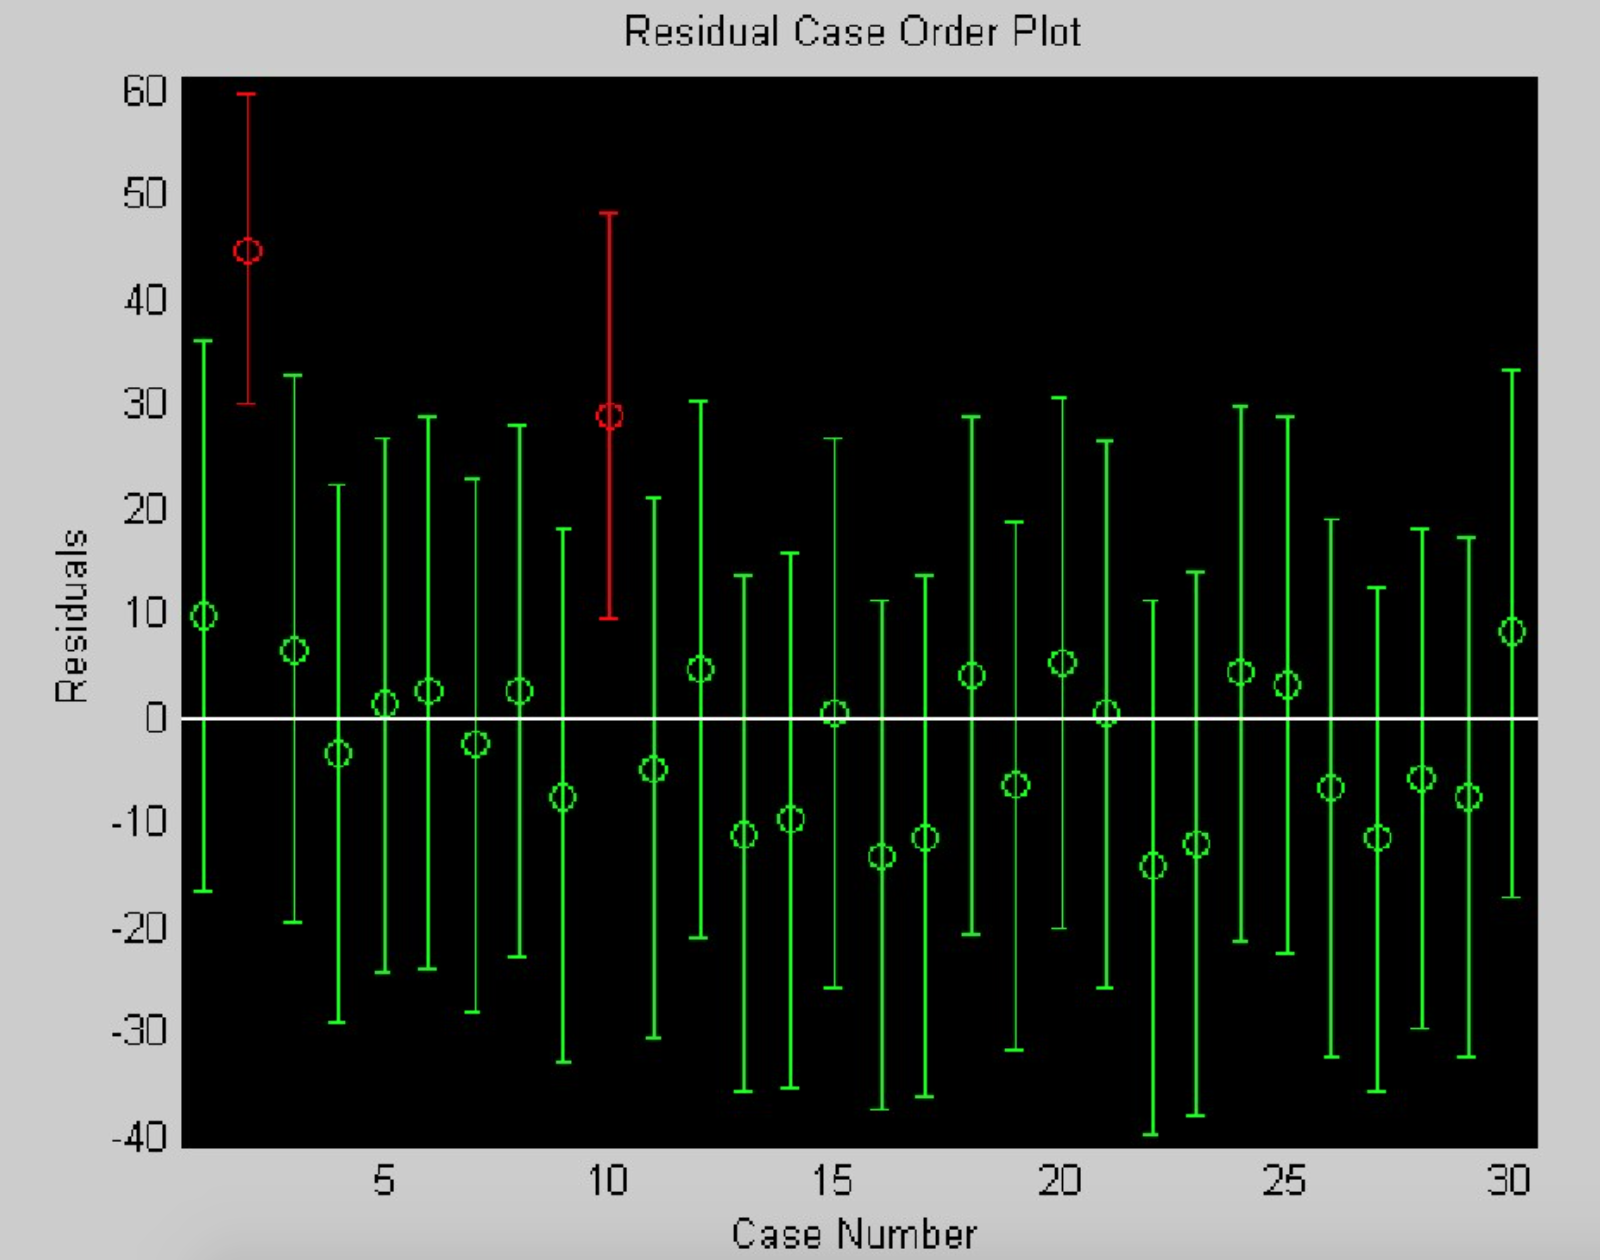
\includegraphics[width=3in]{residual}
  \caption{残差图}
  \label{fig:3.4}
\end{figure}

\subsection{回归方程式变形}
由于有的时候GPS轨迹信息的采样间隔不变,比如有些数据固定隔60s取一个点,直接\ref{f3.9}对采用线性回归的方法由于$T_{total}$不变不能得到满意的效果,所以要对式子进行变形\ref{f3.10}。这样做可以得到两段路的行驶时间,但是只能将路口延迟近似为一个既得的固定值,会对计算的精度造成影响,所以在GPS轨迹信息间隔不固定时还是采用原有的\ref{f3.9}。
\begin{equation}
k_{1} \times T_{1} + k_{2} \times T_{2} + T_{turn} = T_{total}
\label{f3.9}
\end{equation}

\begin{equation}
T_{1} + \frac{k_{2}}{k_{1}} \times T_{2}  = \frac{T_{total} - T_{turn}}{k_{1}}
\label{f3.10}
\end{equation}